\documentclass{article}

\usepackage[a4paper, margin=2cm]{geometry}
\usepackage{amsmath}
\usepackage{amsfonts}
\usepackage{amsthm}
\usepackage{parskip}
\usepackage{xcolor}
\usepackage{graphicx}
\usepackage{amssymb}

\newcommand{\N}{\mathbb{N}}
\newcommand{\Z}{\mathbb{Z}}
\newcommand{\R}{\mathbb{R}}
\newcommand{\DS}[1] {${\displaystyle #1}$}
\newcommand{\st}{\text{ s.t. }}
\newcommand{\de}[1]{\frac{\text{d}}{\text{d}#1}}
\newcommand{\deu}[2]{\frac{\text{d}#2}{\text{d}#1}}
\newcommand{\di}[1]{\text{d}#1}
\newcommand{\code}[1]{\texttt{#1}}
\newcommand{\bigO}{\mathcal{O}}

\title{Project \textit{Breakout} Report}
\author{Fuyang (Scott) Cui}
\date{\today}

\begin{document}
\maketitle 
\tableofcontents
\newpage

\textbf{IMPORTANT: If the game is extremely laggy, please restart the MARS.}

For unknown reasons, MARS starts laggying after few hours of coding and playing.

\section{Memory Layout}

\subsection{Immutable Data}

Part of the memory of my breakout consists of a bunch of immutable data. In my breakout, immutable data are read-only: my breakout never writes to them. We can only change these immutable variables in the source code, and the effects of the changes will reflect in my breakout once the program reruns.

Besides the given \code{ADDR\_DSPL} and \code{ADDR\_KBRD}, I reserved some more memory blocks for the immutable data in my breakout:

\begin{enumerate}
\item \code{WALL\_ATTRIBUTES}.

This variable represents the attributes of the basic building block of my breakout: the walls. I allocated 2 words for this variable and each word stores an integer. 

\begin{itemize}
    \item \code{WALL\_ATTRIBUTES + 0} represents the color of the wall.
    \item \code{WALL\_ATTRIBUTES + 4} represents the thickness of the wall.
\end{itemize}

\item \code{PADDLE\_ATTRIBUTES}.

Similarly, this variable represents the attributes of the paddle in my breakout.

\begin{itemize}
    \item \code{PADDLE\_ATTRIBUTES + 0} represents the color of the paddle.
    \item \code{PADDLE\_ATTRIBUTES + 4} represents the length of the paddle.
    \item \code{PADDLE\_ATTRIBUTES + 8} represents the thickness of the paddle.
\end{itemize}

\item \code{BALL\_ATTRIBUTES}.

This variable represents the attributes of the ball in my breakout.

\begin{itemize}
    \item \code{BALL\_ATTRIBUTES + 0} represents the color of the ball.
    \item \code{BALL\_ATTRIBUTES + 4} represents the radius of the ball.
\end{itemize}

\end{enumerate}

\subsection{Mutable Data}

Most of the \code{.data} section is occupied by mutable data. Mutable data in my breakout are data that may be read and overwritten. Some mutable data may change before executing the instructions, and the effects of those changes will reflect to my breakout once the program reruns.

\begin{enumerate}
\item \code{BRICK\_ATTRIBUTES}

This variable represents the attributes of the bricks. 
\begin{itemize}
    \item \code{BRICK\_ATTRIBUTES + 0} represents the thickness of the bricks.
    \item \code{BRICK\_ATTRIBUTES + 4} represents the number of bricks per row.
    \item \code{BRICK\_ATTRIBUTES + 8} represents the space between rows.
    \item \code{BRICK\_ATTRIBUTES + 12} represents the space between bricks in a row.
    \item \code{BRICK\_ATTRIBUTES + 16} to \code{BRICK\_ATTRIBUTES + 40} represents the colors of rows of bricks from top to bottom. There are 7 colors in total.  
\end{itemize}

\item \code{GAME\_STATUS}

This is an integer signifying the status of the game. \code{GAME\_STATUS == 0} means the game is freezed (paused), and \code{GAME\_STATUS == 1} represents the game is running.

If the game is paused, then the game loop only listens for keyboard inputs. Therefore, no collision detections, objects moving, and screen drawing happen during the freeze.

\item \code{PLAYER\_STATUS}

This is an integer that represents the number of "hearts" the player has. If the heart value drops to 0, then the player dies. 

\item \code{WALL\_AABB}

This variable represents the collision boxes of the walls.

\begin{itemize}
    \item \code{WALL\_AABB + 0} represents the lower bound of the top wall.
    \item \code{WALL\_AABB + 4} represents the right bound of the left wall.
    \item \code{WALL\_AABB + 8} represents the left bound of the right wall.
\end{itemize}

If the ball hit any bound, the collision happens and the ball changes its direction(s). Detailed description of how the ball changes its direction will be illustrated in section 3.

\item \code{BALL\_AABB}

This variable represents the collision box of the ball. This variable is used for detecting collisions and moving the ball.

\begin{itemize}
    \item \code{BALL\_AABB + 0} represents the $x$ position of the upper left corner of the ball. I will denote it as $x_0$ of the ball.
    \item \code{BALL\_AABB + 4} represents the $y$ position of the upper left corner of the ball. I will denote it as $y_0$ of the ball.
    \item \code{BALL\_AABB + 8} represents the $x$ position of the upper right corner of the ball. I will denote it as $x_1$ of the ball.
    \item \code{BALL\_AABB + 8} represents the $y$ position of the lower left corner of the ball. I will denote it as $y_1$ of the ball.
\end{itemize}

\item \code{BALL\_DIRECTION}

This variable represents the direction of the ball. 

\begin{itemize}
    \item \code{BALL\_DIRECTION + 0} represents $x$ direction of the ball. A positive value represents a leftward direction. A negative value represents a rightward direction.
    \item \code{BALL\_DIRECTION + 4} represents $y$ direction of the ball. A positive value represents a downward direction. A negative value represents a upward direction.
\end{itemize}

This variable will be mutated every time the ball changes its direction. The \code{move\_ball} function utilizes this variable and move the ball in the corresponding direction.

\item \code{PADDLE\_AABB}

This variable represents the collision box of the paddle. This variable is used for detecting collisions and moving the paddle.

\begin{itemize}
    \item \code{PADDLE\_AABB + 0} represents the $x$ position of the upper left corner of the paddle. I will denote it as $x_0$ of the paddle.
    \item \code{PADDLE\_AABB + 4} represents the $y$ position of the upper left corner of the paddle. I will denote it as $y_0$ of the paddle.
    \item \code{PADDLE\_AABB + 8} represents the $x$ position of the upper right corner of the paddle. I will denote it as $x_1$ of the paddle.
    \item \code{PADDLE\_AABB + 8} represents the $y$ position of the lower left corner of the paddle. I will denote it as $y_1$ of the paddle.
\end{itemize}

\item \code{BRICKS\_DATA}

This variable represents the data of all bricks. Its capacity depends on the number of bricks we have. I implemented 10 levels and each level has a different number of bricks. Therefore, the design choice is that I allocate the space needed for the maximum number of bricks (1750 integers).

Each brick can be fully characterized in my breakout using 5 integers. The first integer specifies the remaining health of the brick. If the health drops to 0, then the brick disappears. The health is decremented when the ball hit the brick. The 4 integers specify the collision box of the brick as usual.

\item \code{BRICK\_SOUND\_PITCH\_OFFSET}

This variable represents the current pitch offset of the sound generated by colliding bricks.

\item \code{MOVING\_MODE}

This variable represents the movement mode of the ball. 

\begin{itemize}
    \item \code{MOVING\_MODE = 0} represents that the ball will move in a discrete fashion. The player can fully control the ball and move the ball in any direction.
    \item \code{MOVING\_MODE = 1} (default) represents that the ball will move in a continuous fashion with directions specified by \code{BALL\_DIRECTION}. This mode is used in a normal game setting.
\end{itemize}

\end{enumerate}

\subsection{The Stack, Registers, and ...}

The stack and registers have no special usages. I use them as how Prof. Badr taught us to do.

\subsection{The Bitmap Display}

I set the unit width and height for my breakout to 4. Also, the display width is 512 and the display height is 256. Then, I constructed a coordinate system. The coordinate system starts from the left corner (the origin) and ends at the right corner $(128, 0)$ and the lower left corner $(64, 0)$. All variables related to thickness, length, and ... are measured in units.

The \code{draw\_row}, \code{draw\_block\_unit}, and \code{coordinate\_to\_display} functions collaborate together to draw the entire scene out.

\subsection{Screenshots of the Memory}

\begin{figure}[h!]
    \centering
    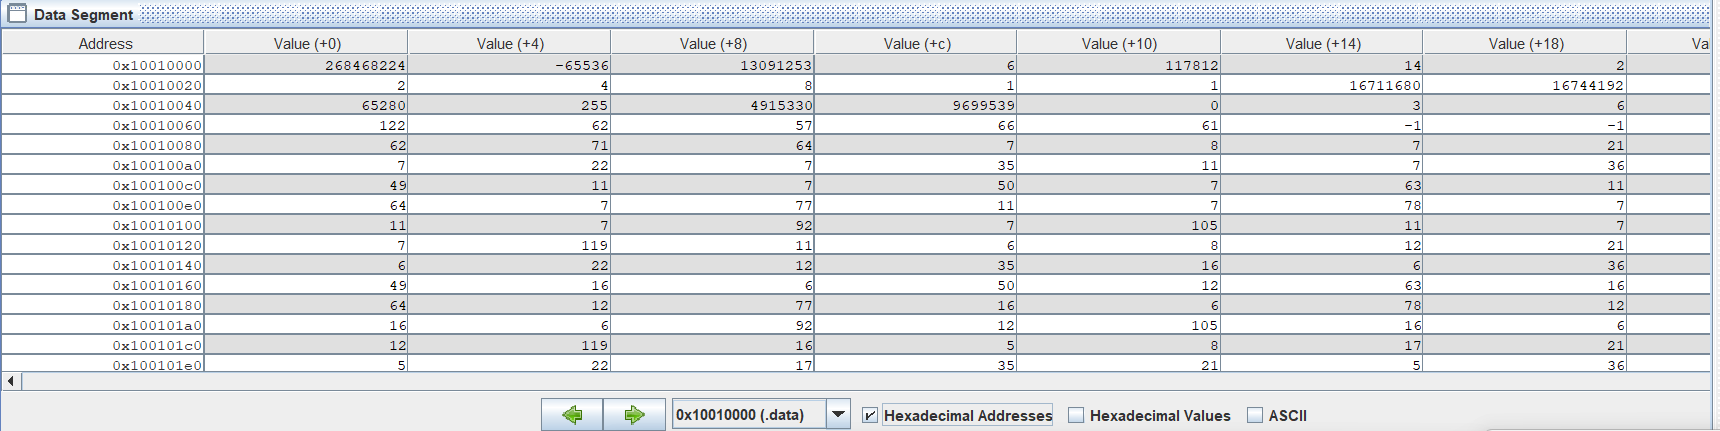
\includegraphics[width=1.0\textwidth]{memory_0.png}
    \caption{A screenshot of the memory of \code{.data} section.}
\end{figure}

As we can observe from Figure 1, data are laid out in the order I introduced.

\begin{figure}[h!]
    \centering
    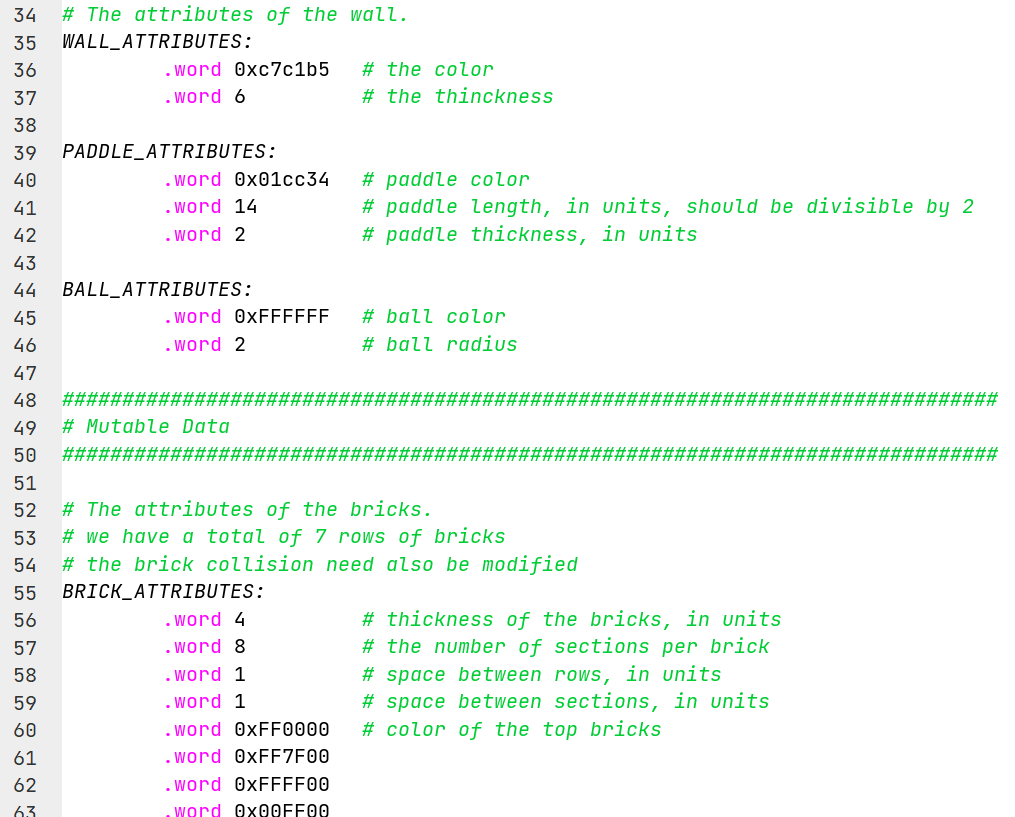
\includegraphics[width=0.6\textwidth]{memory_1.png}
    \caption{A screenshot of the \code{.data} section.}
\end{figure}

\begin{figure}[h!]
    \centering
    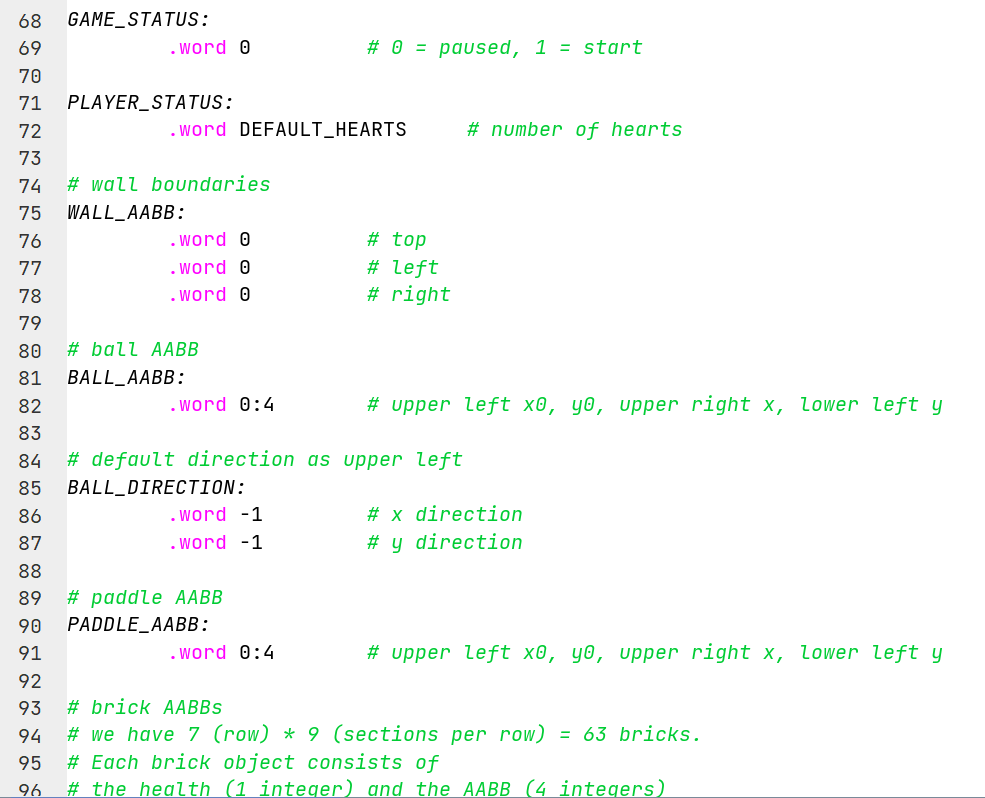
\includegraphics[width=0.6\textwidth]{memory_2.png}
    \caption{A screenshot of the \code{.data} section.}
\end{figure}

\begin{figure}[h!]
    \centering
    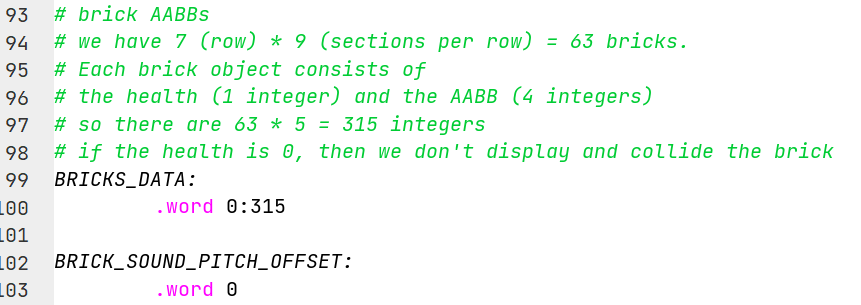
\includegraphics[width=0.6\textwidth]{memory_3.png}
    \caption{A screenshot of the \code{.data} section.}
\end{figure}

\newpage

\section{The Static Scene}

\begin{figure}[h!]
    \centering
    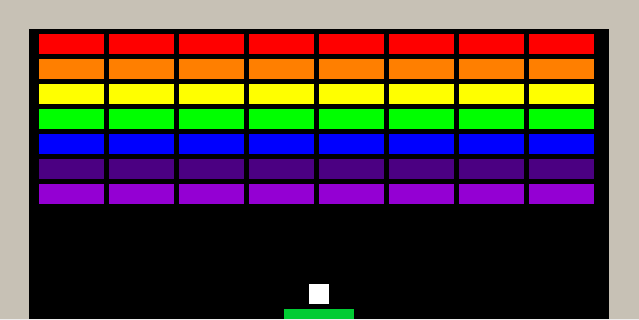
\includegraphics[width=0.8\textwidth]{static_scene_0.png}
    \caption{A screenshot of a static scene of my breakout.}
\end{figure}

\newpage

\section{Collision Detections}

\subsection{The \code{is\_collide} Function}

This function takes two parameters: The address of the first collision box and the address of the second collision box. Collision boxes are specified in section 1.2. This function returns 2 integers: \code{\$v0} specifies if there is a collision between the two collision boxes, and \code{\$v1} specifies the type of the collision if exists, or -1 otherwise.

This function divides collisions into 4 types. For simplicity, let's assume the first parameter is the ball and the second parameter is a brick.

\begin{enumerate}
    \item Type 1: If the ball hit the brick on a horizontal side, the function returns a type 1 collision.
    \begin{figure}[h!]
        \centering
        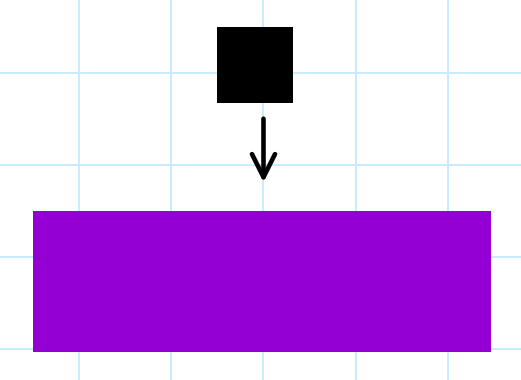
\includegraphics[width=0.2\textwidth]{collision_0.png}
        \caption{A illustration of a Type 1 collision.}
    \end{figure}
    \item Type 2: If the ball hit the brick on a vertical side, the function returns a type 2 collision.
    \begin{figure}[h!]
        \centering
        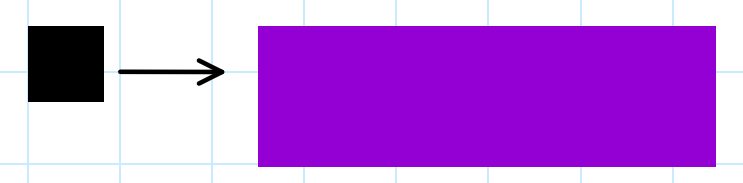
\includegraphics[width=0.2\textwidth]{collision_1.png}
        \caption{A illustration of a Type 2 collision.}
    \end{figure}
    \item Type 3: If the ball hit the brick from a contrary direction on a corner, the function returns a type 3 collision. 
    \begin{figure}[h!]
        \centering
        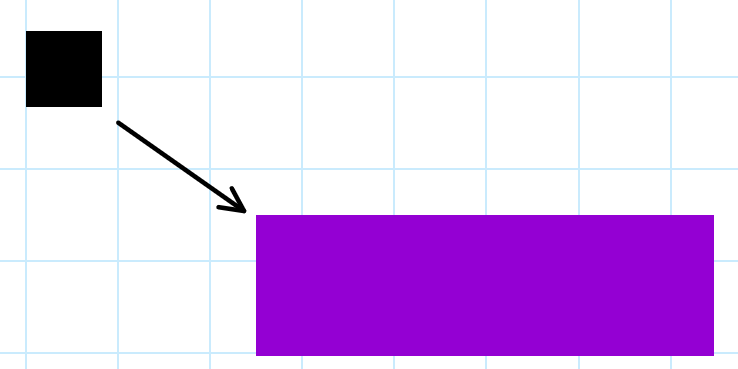
\includegraphics[width=0.2\textwidth]{collision_2.png}
        \caption{A illustration of a Type 3 collision.}
    \end{figure}
    \item Type 4: If the ball hit the brick from the same direction on a corner, the function returns a type 4 collision.
    \begin{figure}[h!]
        \centering
        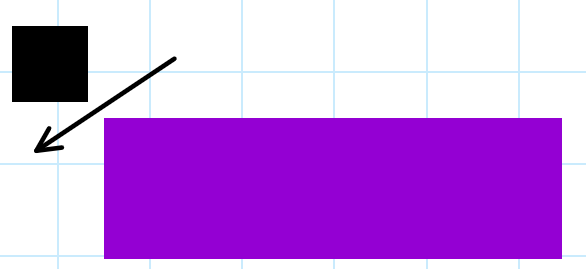
\includegraphics[width=0.2\textwidth]{collision_3.png}
        \caption{A illustration of a Type 4 collision.}
    \end{figure}
\end{enumerate}

\subsection{The Collision Handlers}

Different types of collisions are handled differently.

\begin{enumerate}
    \item For a Type 1 collision, the handler flip the vertical direction of the ball. 
    \begin{figure}[h!]
        \centering
        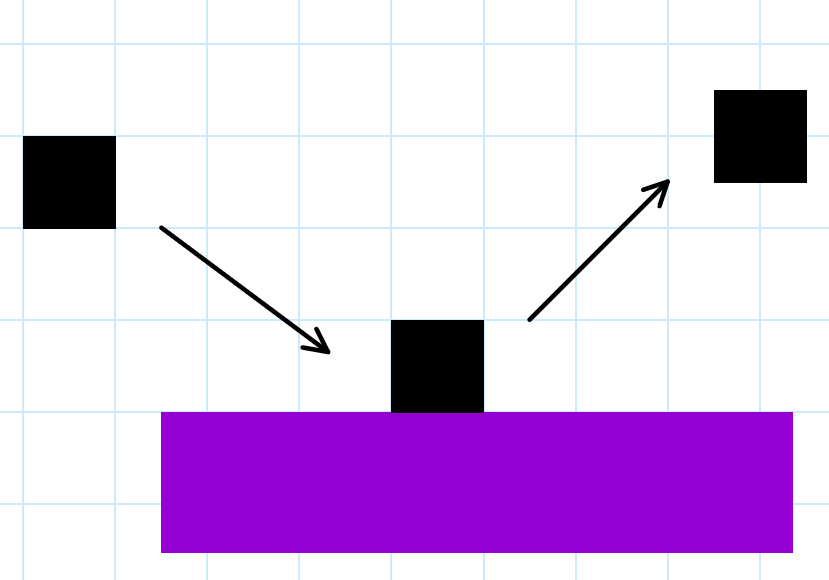
\includegraphics[width=0.2\textwidth]{collision_4.png}
        \caption{A illustration of a Type 1 collision handler.}
    \end{figure}

    \newpage
    
    \item For a Type 2 collision, the handler flip the horizontal direction of the ball.
    \begin{figure}[h!]
        \centering
        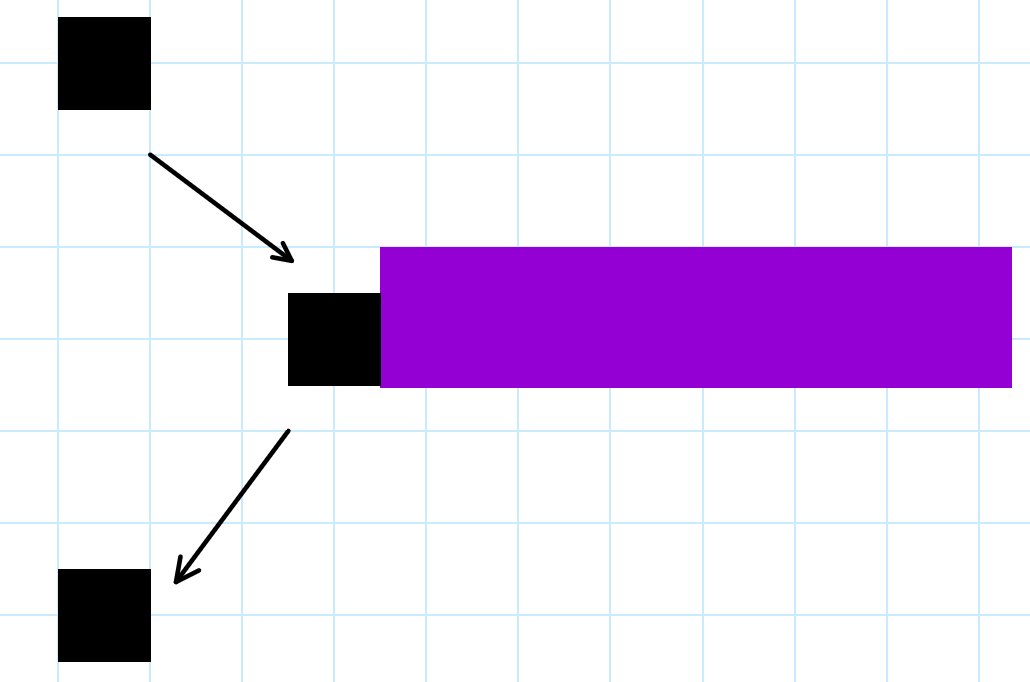
\includegraphics[width=0.2\textwidth]{collision_5.png}
        \caption{A illustration of a Type 2 collision handler.}
    \end{figure}
    \item For a Type 3 collision, the handler flip both the vertical and horizontal directions of the ball. 
    \begin{figure}[h!]
        \centering
        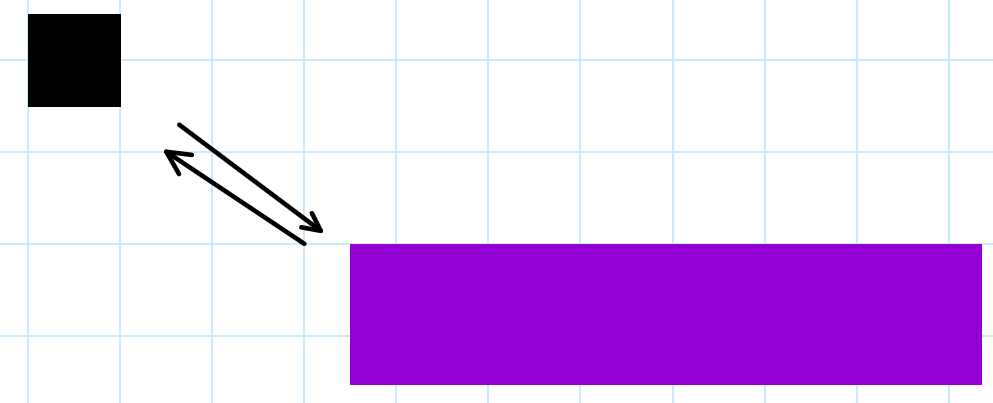
\includegraphics[width=0.2\textwidth]{collision_6.png}
        \caption{A illustration of a Type 3 collision handler.}
    \end{figure}
    \item For a Type 4 collision, the handler doesn't flip any direction.
    \begin{figure}[h!]
        \centering
        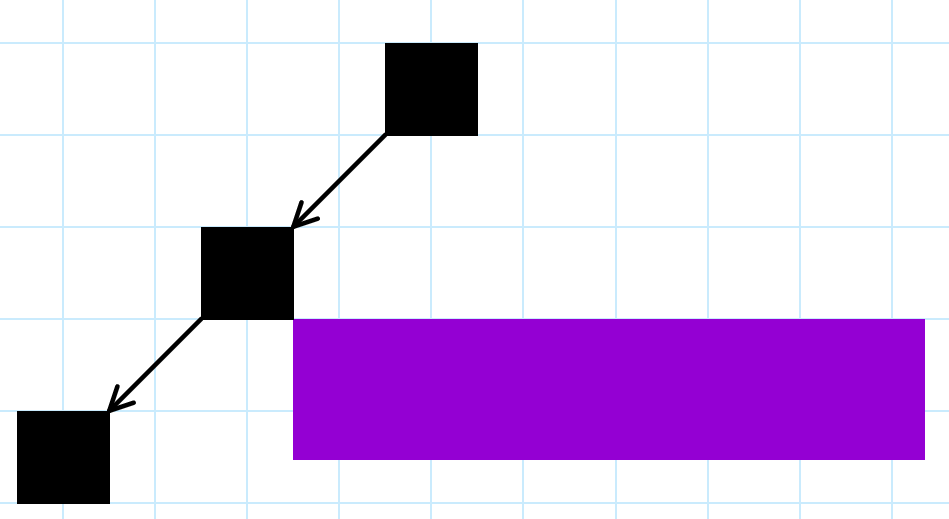
\includegraphics[width=0.2\textwidth]{collision_7.png}
        \caption{A illustration of a Type 4 collision handler.}
    \end{figure}
\end{enumerate}

These illustrations demonstrate my implementation of how will the ball change directions when it collides.

\section{Features}

I implemented easy feature 1, 4, and 5 and hard feature 3 and 4 in the handout.

\subsection{Easy Features}

\begin{enumerate}
    \item[1.] Support ``multiple lives'' (at least 3) so that the player can attempt to make all the bricks disappear multiple times. The state of previous attempts (i.e., broken bricks) should be retained for subsequent attempts.
    
    To implement this feature, I added a new mutable variable: \code{PLAYER\_STATUS}. A detailed description of this variable can be viewed in 1.2 Mutable Data. 
    
    Then, I modified the function \code{move\_ball} which is used to move the ball with directions specified by \code{BALL\_DIRECTION}. If the $y1$ of the ball hits the void, then the function decrements \code{PLAYER\_STATUS}, sleeps for 2 seconds, and then redraws the paddle and the ball at their initial positions. 

    If the \code{PLAYER\_STATUS} was already 1, then the function will quit the game.

    Thus, in this way, the previous attempts are retained and the player can play multiple times. We can set the default value of \code{PLAYER\_STATUS} to $n \in \N$ to give the player $n$ opportunities.

    \item[4.] Add sound effects for different conditions like colliding with the wall, brick, and paddle and for winning and game over.
    
    I added some random sound effects for colliding with the wall and the paddle. Then, I added a variable \code{BRICK\_SOUND\_PITCH\_OFFSET} to record the current offset of the pitch of the sound effect for colliding with a brick. The offset will start from 0 and increment to 24. In this way, a pitch-increasing sequence of piano sounds will be played when the ball collides bricks. 

    \item[5.] Allow the user to pause the game by pressing the keyboard key \code{p}.
    
    To implement this feature, I added a new mutable variable \code{GAME\_STATUS}. A detailed description of this variable can be viewed in 1.2 Mutable Data. 

    If \code{GAME\_STATUS} is 0, then my breakout only processes the keyboard inputs. Therefore, nothing moves if the game is paused. If \code{GAME\_STATUS} is 1, then the game proceeds as normal.

    The keyboard event for the key \code{p} flips the \code{GAME\_STATUS}, so we can use \code{p} to pause/continue the game.
    
\end{enumerate}

\subsection{Hard Features}

\begin{enumerate}
    \item[3.] Require bricks be hit by the ball multiple times before breaking. Demonstrate the players progress toward breaking a brick in some way (e.g., different colours).
    
    In \code{BRICKS\_DATA} variable (detailed description in 1.2 Mutable Data), each brick is associated with a health value. A collision will cause the health value of the collided brick decrement. Once the health value hit 0, the brick is considered broken, the brick won't be drawn again, and the collision box of it is considered invalid.

    Thus, I modified the collision detection loops and the function to redraw the bricks to support the functionality.

    I defined the top row of bricks has the highest initial health value (7) and the bottom row of bricks has the lowest initial health value (1). I associated the health values with the colors of the brick. Low-health bricks are displayed in bottom-row color and high-health bricks are displayed in top-row color.
    \begin{figure}[h!]
        \centering
        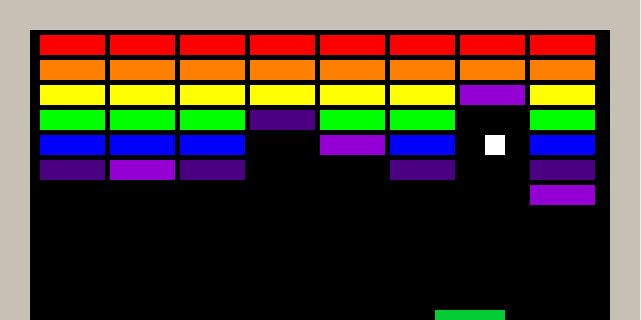
\includegraphics[width=0.8\textwidth]{feature_0.png}
        \caption{A illustration of the hard feature.}
    \end{figure}
    \item[4.] Create a second level with a different layout of bricks.
    
    With the help of \code{BRICK\_ATTRIBUTES}, I can create different layouts easily.

    I define layout 1 to be 1 brick per row, layout 2 to be 2 bricks per row, and ....

    I added some keyboard listeners for keys \code{1}, \code{2}, .... Each listener pauses the current game, reset the display, update the brick attributes, reset the player's status, and finally reinitialize to the new layout. Therefore, I can switch to different levels anytime I want.
    \begin{figure}[h!]
        \centering
        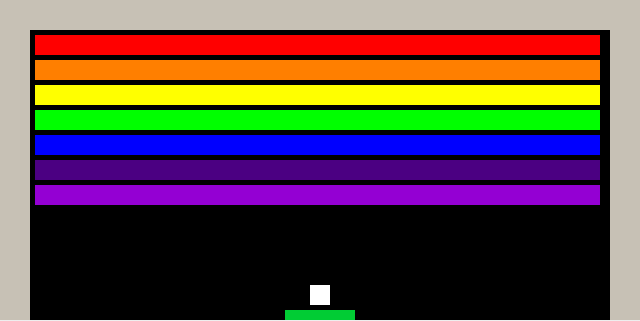
\includegraphics[width=0.8\textwidth]{level_1.png}
        \caption{A illustration of the level 1 layout.}
    \end{figure}
    \begin{figure}[h!]
        \centering
        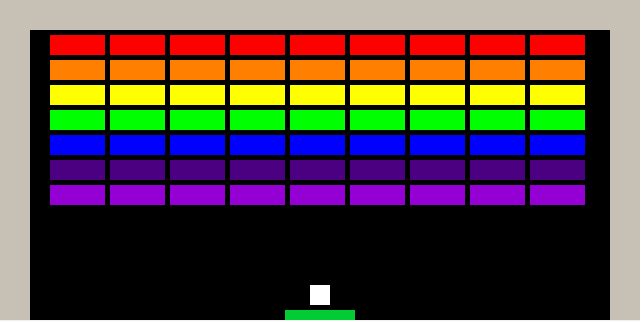
\includegraphics[width=0.8\textwidth]{level_9.png}
        \caption{A illustration of the level 9 layout.}
    \end{figure}
    \begin{figure}[h!]
        \centering
        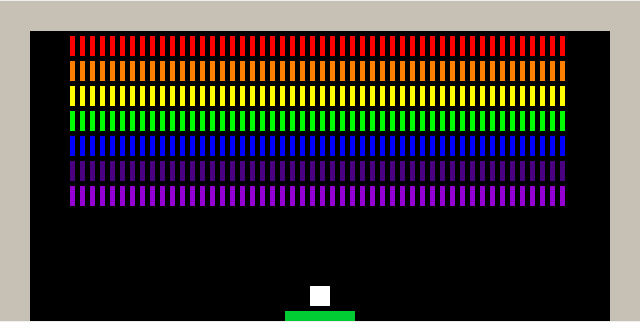
\includegraphics[width=0.8\textwidth]{level_0.png}
        \caption{A illustration of the level mysterious layout.}
    \end{figure}


\end{enumerate}

\newpage

\section{How to play?}

\textbf{IMPORTANT: If the game is extremely laggy, please restart the MARS.}

For unknown reasons, MARS starts laggying after few hours of coding and playing.

There are 3 modes in total to play. 

Before playing in any mode, please set the bitmap display as in the preamble.
\begin{itemize}
    \item Unit Width in Pixels = 4
    \item Unit Height in Pixels = 4
    \item Display Width in Pixels = 512
    \item Display Height in Pixels = 256
    \item Base address for display = 0x10008000 (\$gp)
\end{itemize}

\subsection{Normal Mode}

To play the Normal Mode, please set the equivalences to the followings:

\begin{itemize}
    \item \code{.eqv AUTO\_MODE 0}
    \item \code{.eqv SLEEP 32} (if you feel very hard to play with, feel free to sleep longer)
    \item \code{.eqv DEFAULT\_HEARTS 3} (if you feel very hard to play with, feel free to add more hearts)
    \item \code{.eqv\ DEFAULT\_MOVING\_MODE\ 1}
\end{itemize}

Operations:
\begin{itemize}
    \item \code{s}: Starts the game.
    \item \code{p}: Pauses/continues the game.
    \item \code{q}: Quits the game.
    \item \code{a}: Moves the paddle leftward.
    \item \code{d}: Moves the paddle rightward.
    \item \code{1-9}: Changes level number 1 - 9.
    \item \code{0}: Changes to a mostly unplayable level.
\end{itemize}

Notes: 
\begin{itemize}
    \item After changing the level, you need to press \code{s} to start the game.
    \item You can change to different levels anytime you want.
    \item The game will quit automatically if you lose.
    \item After a failure, if you have at least one more heart, you will respawn after 2 seconds. Then, you need to press \code{s} to resume the game.
\end{itemize}

\subsection{Automatic Mode}

In this mode, the paddle follows the ball automatically.

To play the automatic mode, please set the equivalences to the followings:

\begin{itemize}
    \item \code{.eqv AUTO\_MODE 1}
    \item \code{.eqv SLEEP 0} (basically, any sleep values you want: the smaller, the faster)
    \item \code{.eqv DEFAULT\_HEARTS 1} (any integer greater than or equal to 1)
    \item \code{.eqv\ DEFAULT\_MOVING\_MODE\ 1}
\end{itemize}

\subsection{God Mode}

In the God Mode, you can use keys to fully control the movement of the ball.

To play the god mode, please set the equivalences to the followings:

\begin{itemize}
    \item \code{.eqv AUTO\_MODE 1}
    \item \code{.eqv SLEEP 0} (basically, any sleep values you want: the smaller, the faster)
    \item \code{.eqv DEFAULT\_HEARTS 1} (any integer greater than or equal to 1)
    \item \code{.eqv\ DEFAULT\_MOVING\_MODE\ 0}
\end{itemize}

Operations (in addition to operations in the Normal Mode):
\begin{itemize}
    \item \code{i}: Moves the ball upward 1 unit. 
    \item \code{j}: Moves the ball leftward 1 unit. 
    \item \code{k}: Moves the ball downward 1 unit. 
    \item \code{l}: Moves the ball rightward 1 unit. 
    \item \code{u}: Moves the ball up-leftward 1 unit. 
    \item \code{o}: Moves the ball up-rightward 1 unit. 
    \item \code{m}: Moves the ball down-leftward 1 unit. 
    \item \code{.}: Moves the ball down-rightward 1 unit. 
    \item \code{,}: Resets the directions of the ball to no direction. ($(0, 0)$ for $x$ and $y$ directions)
    \item \code{n}: Flips the moving mode (see 1.2 Mutable Data). 
\end{itemize}

\end{document}